\section{Database}
\subsection{Descrizione}
sqlite3
\subsection{Modello E/R}
\begin{figure}[ht]
    \centering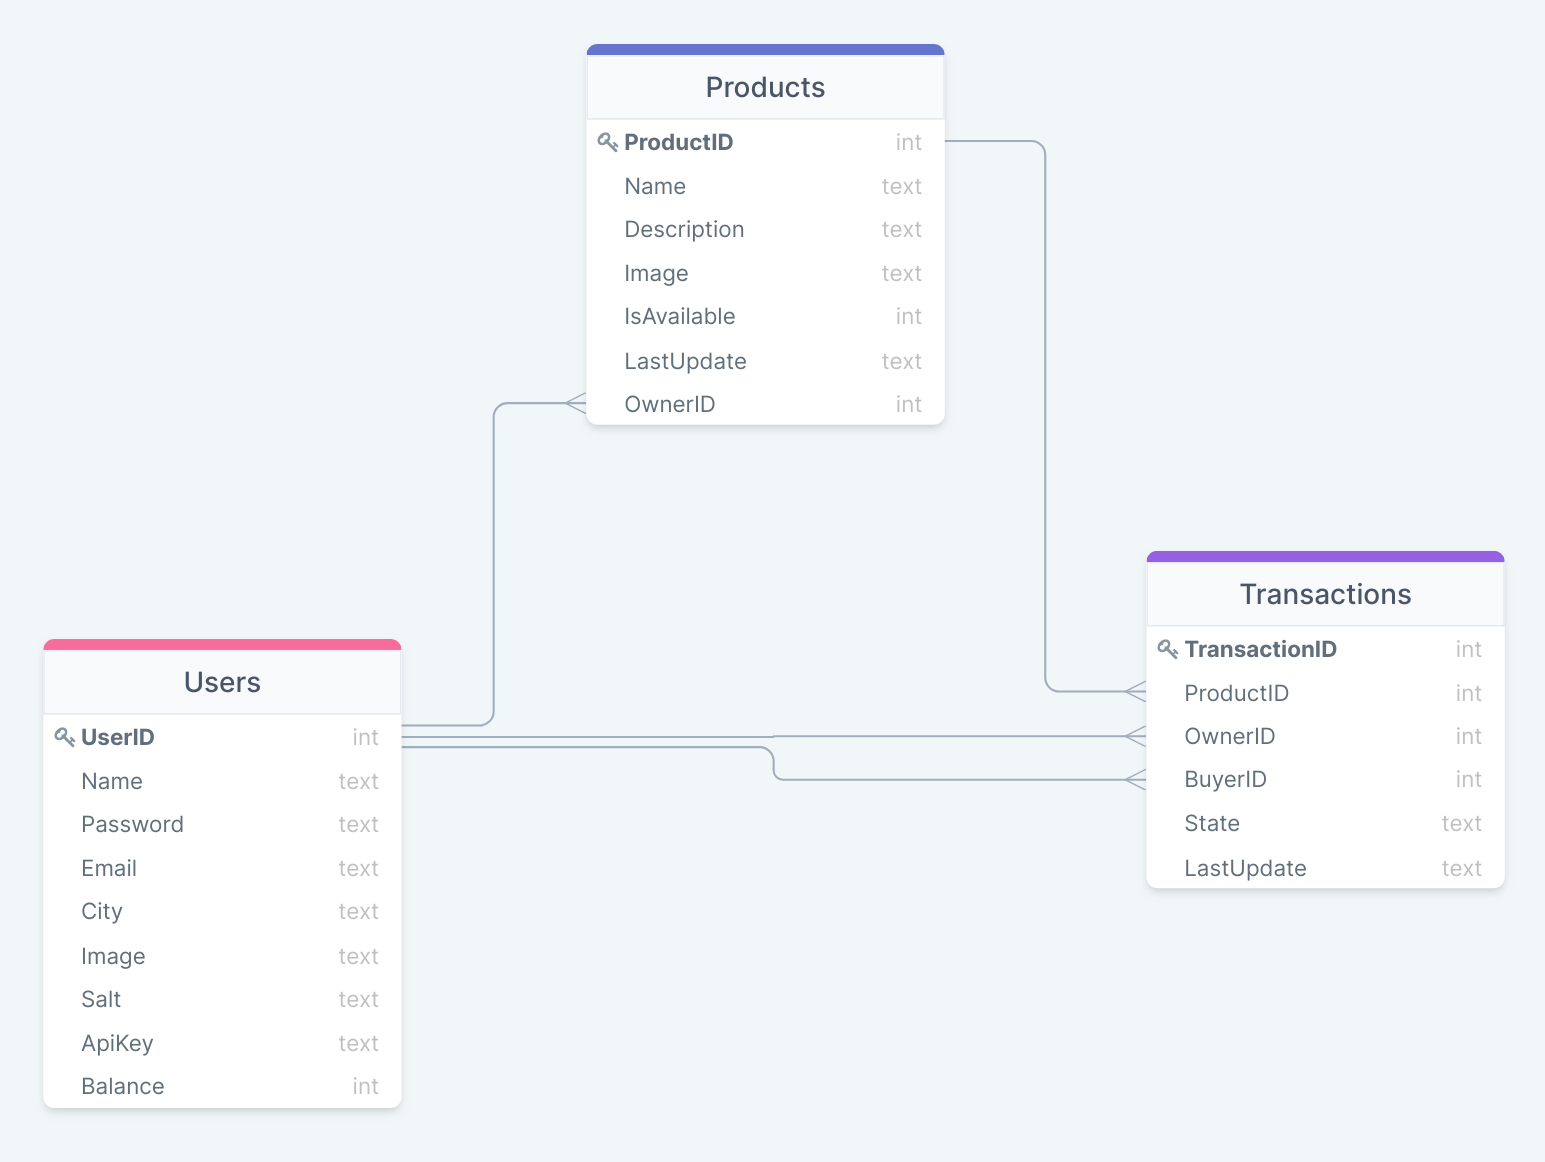
\includegraphics[scale=0.29]{images/modello_e_r.png}
    \caption{Modello E/R del database}
\end{figure}
\subsection{Modello logico}
\begin{figure}[ht]
    \centering\begin{tabular}{ |l|c|l| } 
    \hline
    \multicolumn{3}{|c|}{\large\textbf{Users}} \\
    \hline
    \textbf{Nome Campo} & \textbf{Tipo} & \textbf{Note} \\
    \hline
    UserID & INTEGER & NOT NULL, PK \\
    Name & TEXT & NOT NULL \\
    Password & TEXT & NOT NULL \\
    Email & TEXT & NOT NULL \\
    City & TEXT & NOT NULL \\
    Image & TEXT & NOT NULL \\
    Salt & TEXT & NOT NULL \\
    ApiKey & TEXT & NOT NULL \\
    Balance & INTEGER & NOT NULL \\
    \hline
    \end{tabular}
    \caption{Tabella Users parte del modello logico del database}
\end{figure}
\begin{figure}[ht]
    \centering\begin{tabular}{ |l|c|l| } 
    \hline
    \multicolumn{3}{|c|}{\large\textbf{Products}} \\
    \hline
    \textbf{Nome Campo} & \textbf{Tipo} & \textbf{Note} \\
    \hline
    ProductID & INTEGER & NOT NULL, PK \\
    Name & TEXT & NOT NULL \\
    Description & TEXT & NOT NULL \\
    Image & TEXT & NOT NULL \\
    IsAvailable & INTEGER & NOT NULL \\
    LastUpdate & TEXT & NOT NULL \\
    OwnerID & INTEGER & NOT NULL, FK(Users) \\
    \hline
    \end{tabular}
    \caption{Tabella Products parte del modello logico del database}
\end{figure}
\begin{figure}[ht]
    \centering\begin{tabular}{ |l|c|l| } 
    \hline
    \multicolumn{3}{|c|}{\large\textbf{Transactions}} \\
    \hline
    \textbf{Nome Campo} & \textbf{Tipo} & \textbf{Note} \\
    \hline
    TransactionID & INTEGER & NOT NULL, PK \\
    ProductID & INTEGER & NOT NULL, FK(Products) \\
    OwnerID & INTEGER & NOT NULL, FK(Users) \\
    BuyerID & INTEGER & NOT NULL, FK(Users) \\
    State & TEXT & NOT NULL \\
    LastUpdate & TEXT & NOT NULL \\
    \hline
    \end{tabular}
    \caption{Tabella Transactions parte del modello logico del database}
\end{figure}
\subsection{Entity Framework Core}
db schema generato code-first
code snippets